% Figura Anexo II: la lotería de CALVO y su huella en la pendiente de la curva de PHILLIPS
\documentclass[tikz,border=3pt]{standalone}
\usepackage[T1]{fontenc}
\usepackage[utf8]{inputenc}
\usepackage{amsmath}
\usetikzlibrary{arrows.meta,calc,positioning}
\begin{document}
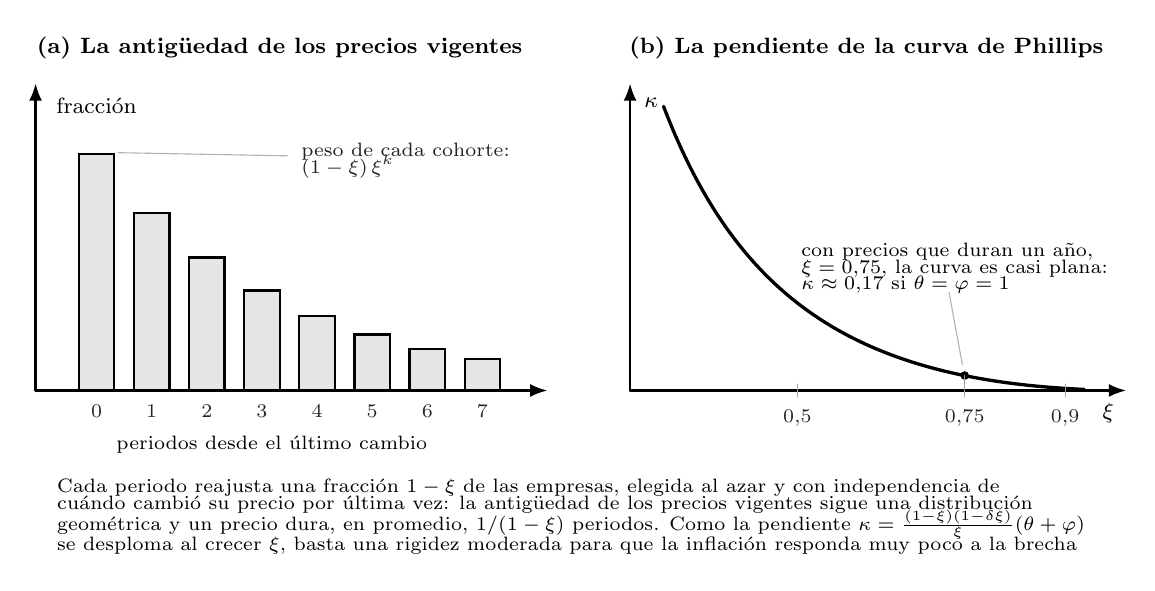
\begin{tikzpicture}[>={Latex[length=2.2mm]}, line cap=round, font=\footnotesize,
  eje/.style={->, thick},
  curva/.style={very thick},
  barra/.style={fill=black!10, draw=black, thick},
  guia/.style={densely dashed, gray!80},
  pto/.style={circle, fill=black, inner sep=1.1pt}]
  % ---------- Panel (a): la loteria ----------
  \node[font=\footnotesize\bfseries] at (3.1,4.35) {(a) La antigüedad de los precios vigentes};
  \draw[eje] (0,0) -- (6.5,0);
  \node[font=\scriptsize, anchor=north] at (3.0,-0.46) {periodos desde el último cambio};
  \draw[eje] (0,0) -- (0,3.9) node[below right=2pt]{\;fracción};
  \foreach \k/\x/\h in {0/0.55/3.00, 1/1.25/2.25, 2/1.95/1.69, 3/2.65/1.27, 4/3.35/0.95, 5/4.05/0.71, 6/4.75/0.53, 7/5.45/0.40}{
    \draw[barra] (\x,0) rectangle (\x+0.45,\h);
    \node[font=\scriptsize, anchor=north, gray!30!black] at (\x+0.225,-0.06) {\k};
  }
  \node[anchor=west, font=\scriptsize, align=left, gray!25!black] at (3.25,2.92)
    {peso de cada cohorte:\\[-2pt]$\left(1-\xi\right)\xi^{k}$};
  \draw[gray!60] (3.2,2.98) -- (1.05,3.02);
  % ---------- Panel (b): la pendiente ----------
  \begin{scope}[xshift=7.55cm]
    \node[font=\footnotesize\bfseries] at (3.0,4.35) {(b) La pendiente de la curva de \textsc{Phillips}};
    \draw[eje] (0,0) -- (6.3,0) node[below left=1pt]{$\xi$};
    \draw[eje] (0,0) -- (0,3.9) node[below right=2pt]{$\kappa$};
    \draw[curva, domain=0.30:0.93, samples=90, smooth] plot ({(\x-0.25)*8.5},{2*(1-\x)*(1-0.99*\x)/\x*1.1});
    \foreach \v/\t in {0.5/{$0{,}5$}, 0.75/{$0{,}75$}, 0.9/{$0{,}9$}}{
      \pgfmathsetmacro{\xc}{(\v-0.25)*8.5}
      \draw[gray!70] (\xc,-0.08) -- (\xc,0.08);
      \node[font=\scriptsize, anchor=north, gray!30!black] at (\xc,-0.12) {\t};
    }
    \node[pto] (K75) at (4.25,0.19) {};
    \draw[guia] (4.25,0.19) -- (4.25,0);
    \node[anchor=west, font=\scriptsize, align=left] at (2.05,1.55)
      {con precios que duran un año,\\[-2pt]$\xi=0{,}75$, la curva es casi plana:\\[-2pt]$\kappa\approx 0{,}17$ si $\theta=\varphi=1$};
    \draw[gray!60] (4.05,1.25) -- (4.22,0.33);
  \end{scope}
  \node[align=left, anchor=north west, font=\scriptsize] at (0.15,-1.0)
    {Cada periodo reajusta una fracción $1-\xi$ de las empresas, elegida al azar y con independencia de\\[-2pt]cuándo cambió su precio por última vez: la antigüedad de los precios vigentes sigue una distribución\\[-2pt]geométrica y un precio dura, en promedio, $1/(1-\xi)$ periodos. Como la pendiente $\kappa=\frac{(1-\xi)(1-\delta\xi)}{\xi}(\theta+\varphi)$\\[-2pt]se desploma al crecer $\xi$, basta una rigidez moderada para que la inflación responda muy poco a la brecha};
\end{tikzpicture}
\end{document}
